% Created by tikzDevice version 0.10.1 on 2016-08-15 14:36:25
% !TEX encoding = UTF-8 Unicode
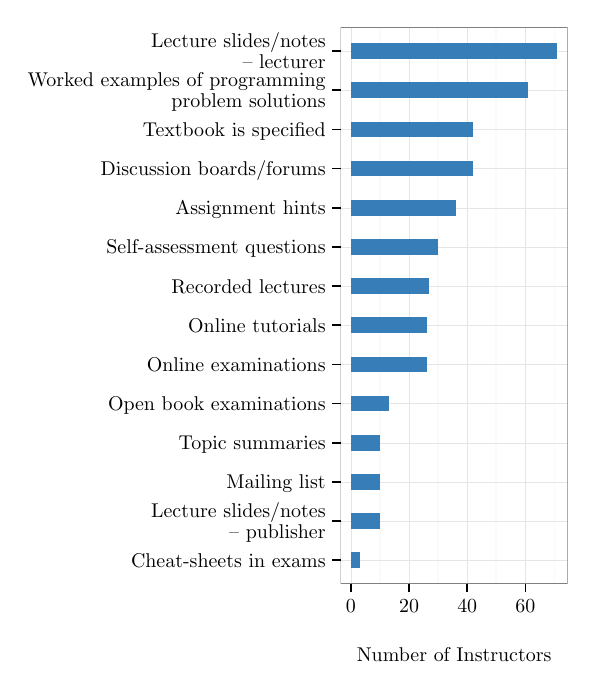
\begin{tikzpicture}[x=1pt,y=1pt]
\definecolor{fillColor}{RGB}{255,255,255}
\path[use as bounding box,fill=fillColor,fill opacity=0.00] (0,0) rectangle (195.13,231.26);
\begin{scope}
\path[clip] (  0.00,  0.00) rectangle (195.13,231.26);
\definecolor{drawColor}{RGB}{255,255,255}
\definecolor{fillColor}{RGB}{255,255,255}

\path[draw=drawColor,line width= 0.6pt,line join=round,line cap=round,fill=fillColor] (  0.00,  0.00) rectangle (195.13,231.26);
\end{scope}
\begin{scope}
\path[clip] (113.07, 30.29) rectangle (195.13,231.26);
\definecolor{fillColor}{RGB}{255,255,255}

\path[fill=fillColor] (113.07, 30.29) rectangle (195.13,231.26);
\definecolor{drawColor}{gray}{0.98}

\path[draw=drawColor,line width= 0.6pt,line join=round] (127.31, 30.29) --
	(127.31,231.26);

\path[draw=drawColor,line width= 0.6pt,line join=round] (148.32, 30.29) --
	(148.32,231.26);

\path[draw=drawColor,line width= 0.6pt,line join=round] (169.34, 30.29) --
	(169.34,231.26);

\path[draw=drawColor,line width= 0.6pt,line join=round] (190.35, 30.29) --
	(190.35,231.26);
\definecolor{drawColor}{gray}{0.90}

\path[draw=drawColor,line width= 0.2pt,line join=round] (113.07, 38.79) --
	(195.13, 38.79);

\path[draw=drawColor,line width= 0.2pt,line join=round] (113.07, 52.94) --
	(195.13, 52.94);

\path[draw=drawColor,line width= 0.2pt,line join=round] (113.07, 67.09) --
	(195.13, 67.09);

\path[draw=drawColor,line width= 0.2pt,line join=round] (113.07, 81.24) --
	(195.13, 81.24);

\path[draw=drawColor,line width= 0.2pt,line join=round] (113.07, 95.40) --
	(195.13, 95.40);

\path[draw=drawColor,line width= 0.2pt,line join=round] (113.07,109.55) --
	(195.13,109.55);

\path[draw=drawColor,line width= 0.2pt,line join=round] (113.07,123.70) --
	(195.13,123.70);

\path[draw=drawColor,line width= 0.2pt,line join=round] (113.07,137.86) --
	(195.13,137.86);

\path[draw=drawColor,line width= 0.2pt,line join=round] (113.07,152.01) --
	(195.13,152.01);

\path[draw=drawColor,line width= 0.2pt,line join=round] (113.07,166.16) --
	(195.13,166.16);

\path[draw=drawColor,line width= 0.2pt,line join=round] (113.07,180.31) --
	(195.13,180.31);

\path[draw=drawColor,line width= 0.2pt,line join=round] (113.07,194.47) --
	(195.13,194.47);

\path[draw=drawColor,line width= 0.2pt,line join=round] (113.07,208.62) --
	(195.13,208.62);

\path[draw=drawColor,line width= 0.2pt,line join=round] (113.07,222.77) --
	(195.13,222.77);

\path[draw=drawColor,line width= 0.2pt,line join=round] (116.80, 30.29) --
	(116.80,231.26);

\path[draw=drawColor,line width= 0.2pt,line join=round] (137.82, 30.29) --
	(137.82,231.26);

\path[draw=drawColor,line width= 0.2pt,line join=round] (158.83, 30.29) --
	(158.83,231.26);

\path[draw=drawColor,line width= 0.2pt,line join=round] (179.84, 30.29) --
	(179.84,231.26);
\definecolor{fillColor}{RGB}{55,126,184}

\path[fill=fillColor] (116.80, 35.95) rectangle (119.96, 41.62);

\path[fill=fillColor] (116.80, 50.11) rectangle (127.31, 55.77);

\path[fill=fillColor] (116.80, 64.26) rectangle (127.31, 69.92);

\path[fill=fillColor] (116.80, 78.41) rectangle (127.31, 84.07);

\path[fill=fillColor] (116.80, 92.57) rectangle (130.46, 98.23);

\path[fill=fillColor] (116.80,106.72) rectangle (144.12,112.38);

\path[fill=fillColor] (116.80,120.87) rectangle (144.12,126.53);

\path[fill=fillColor] (116.80,135.02) rectangle (145.17,140.69);

\path[fill=fillColor] (116.80,149.18) rectangle (148.32,154.84);

\path[fill=fillColor] (116.80,163.33) rectangle (154.63,168.99);

\path[fill=fillColor] (116.80,177.48) rectangle (160.93,183.14);

\path[fill=fillColor] (116.80,191.64) rectangle (160.93,197.30);

\path[fill=fillColor] (116.80,205.79) rectangle (180.89,211.45);

\path[fill=fillColor] (116.80,219.94) rectangle (191.40,225.60);
\definecolor{drawColor}{gray}{0.50}

\path[draw=drawColor,line width= 0.6pt,line join=round,line cap=round] (113.07, 30.29) rectangle (195.13,231.26);
\end{scope}
\begin{scope}
\path[clip] (  0.00,  0.00) rectangle (195.13,231.26);
\definecolor{drawColor}{RGB}{0,0,0}

\node[text=drawColor,anchor=base east,inner sep=0pt, outer sep=0pt, scale=  0.72] at (107.67, 36.31) {Cheat-sheets in exams};

\node[text=drawColor,anchor=base east,inner sep=0pt, outer sep=0pt, scale=  0.72] at (107.67, 54.35) {Lecture slides/notes};

\node[text=drawColor,anchor=base east,inner sep=0pt, outer sep=0pt, scale=  0.72] at (107.67, 46.57) {-- publisher};

\node[text=drawColor,anchor=base east,inner sep=0pt, outer sep=0pt, scale=  0.72] at (107.67, 64.61) {Mailing list};

\node[text=drawColor,anchor=base east,inner sep=0pt, outer sep=0pt, scale=  0.72] at (107.67, 78.76) {Topic summaries};

\node[text=drawColor,anchor=base east,inner sep=0pt, outer sep=0pt, scale=  0.72] at (107.67, 92.92) {Open book examinations};

\node[text=drawColor,anchor=base east,inner sep=0pt, outer sep=0pt, scale=  0.72] at (107.67,107.07) {Online examinations};

\node[text=drawColor,anchor=base east,inner sep=0pt, outer sep=0pt, scale=  0.72] at (107.67,121.22) {Online tutorials};

\node[text=drawColor,anchor=base east,inner sep=0pt, outer sep=0pt, scale=  0.72] at (107.67,135.38) {Recorded lectures};

\node[text=drawColor,anchor=base east,inner sep=0pt, outer sep=0pt, scale=  0.72] at (107.67,149.53) {Self-assessment questions};

\node[text=drawColor,anchor=base east,inner sep=0pt, outer sep=0pt, scale=  0.72] at (107.67,163.68) {Assignment hints};

\node[text=drawColor,anchor=base east,inner sep=0pt, outer sep=0pt, scale=  0.72] at (107.67,177.83) {Discussion boards/forums};

\node[text=drawColor,anchor=base east,inner sep=0pt, outer sep=0pt, scale=  0.72] at (107.67,191.99) {Textbook is specified};

\node[text=drawColor,anchor=base east,inner sep=0pt, outer sep=0pt, scale=  0.72] at (107.67,210.03) {Worked examples of programming};

\node[text=drawColor,anchor=base east,inner sep=0pt, outer sep=0pt, scale=  0.72] at (107.67,202.25) {problem solutions};

\node[text=drawColor,anchor=base east,inner sep=0pt, outer sep=0pt, scale=  0.72] at (107.67,224.18) {Lecture slides/notes};

\node[text=drawColor,anchor=base east,inner sep=0pt, outer sep=0pt, scale=  0.72] at (107.67,216.40) {-- lecturer};
\end{scope}
\begin{scope}
\path[clip] (  0.00,  0.00) rectangle (195.13,231.26);
\definecolor{drawColor}{RGB}{0,0,0}

\path[draw=drawColor,line width= 0.6pt,line join=round] (110.07, 38.79) --
	(113.07, 38.79);

\path[draw=drawColor,line width= 0.6pt,line join=round] (110.07, 52.94) --
	(113.07, 52.94);

\path[draw=drawColor,line width= 0.6pt,line join=round] (110.07, 67.09) --
	(113.07, 67.09);

\path[draw=drawColor,line width= 0.6pt,line join=round] (110.07, 81.24) --
	(113.07, 81.24);

\path[draw=drawColor,line width= 0.6pt,line join=round] (110.07, 95.40) --
	(113.07, 95.40);

\path[draw=drawColor,line width= 0.6pt,line join=round] (110.07,109.55) --
	(113.07,109.55);

\path[draw=drawColor,line width= 0.6pt,line join=round] (110.07,123.70) --
	(113.07,123.70);

\path[draw=drawColor,line width= 0.6pt,line join=round] (110.07,137.86) --
	(113.07,137.86);

\path[draw=drawColor,line width= 0.6pt,line join=round] (110.07,152.01) --
	(113.07,152.01);

\path[draw=drawColor,line width= 0.6pt,line join=round] (110.07,166.16) --
	(113.07,166.16);

\path[draw=drawColor,line width= 0.6pt,line join=round] (110.07,180.31) --
	(113.07,180.31);

\path[draw=drawColor,line width= 0.6pt,line join=round] (110.07,194.47) --
	(113.07,194.47);

\path[draw=drawColor,line width= 0.6pt,line join=round] (110.07,208.62) --
	(113.07,208.62);

\path[draw=drawColor,line width= 0.6pt,line join=round] (110.07,222.77) --
	(113.07,222.77);
\end{scope}
\begin{scope}
\path[clip] (  0.00,  0.00) rectangle (195.13,231.26);
\definecolor{drawColor}{RGB}{0,0,0}

\path[draw=drawColor,line width= 0.6pt,line join=round] (116.80, 27.29) --
	(116.80, 30.29);

\path[draw=drawColor,line width= 0.6pt,line join=round] (137.82, 27.29) --
	(137.82, 30.29);

\path[draw=drawColor,line width= 0.6pt,line join=round] (158.83, 27.29) --
	(158.83, 30.29);

\path[draw=drawColor,line width= 0.6pt,line join=round] (179.84, 27.29) --
	(179.84, 30.29);
\end{scope}
\begin{scope}
\path[clip] (  0.00,  0.00) rectangle (195.13,231.26);
\definecolor{drawColor}{RGB}{0,0,0}

\node[text=drawColor,anchor=base,inner sep=0pt, outer sep=0pt, scale=  0.72] at (116.80, 19.93) {0};

\node[text=drawColor,anchor=base,inner sep=0pt, outer sep=0pt, scale=  0.72] at (137.82, 19.93) {20};

\node[text=drawColor,anchor=base,inner sep=0pt, outer sep=0pt, scale=  0.72] at (158.83, 19.93) {40};

\node[text=drawColor,anchor=base,inner sep=0pt, outer sep=0pt, scale=  0.72] at (179.84, 19.93) {60};
\end{scope}
\begin{scope}
\path[clip] (  0.00,  0.00) rectangle (195.13,231.26);
\definecolor{drawColor}{RGB}{0,0,0}

\node[text=drawColor,anchor=base,inner sep=0pt, outer sep=0pt, scale=  0.72] at (154.10, 10.18) {};

\node[text=drawColor,anchor=base,inner sep=0pt, outer sep=0pt, scale=  0.72] at (154.10,  2.40) {Number of Instructors};
\end{scope}
\end{tikzpicture}
